
\documentclass{whureport}
\usepackage{booktabs}%三线表
\usepackage{setspace}
\usepackage{stfloats}
\usepackage{graphicx}
\usepackage{datetime}
\usepackage{amsmath}
\usepackage{fancyhdr}
\usepackage{caption}
\usepackage{makecell}
\usepackage{siunitx} % For \SI command
\usepackage[backend=biber,sorting = none]{biblatex}
\addbibresource{article.bib}
\usepackage[breaklinks,colorlinks,linkcolor=black,
citecolor=black,urlcolor=black]{hyperref}
\newcommand{\major}{物理学}
\newcommand{\name}{郑晓旸}
\newcommand{\stuid}{202111030007}
\newcommand{\Name}{Zheng Xiaoyang}
\newcommand{\loc}{None}
\newcommand{\course}{近代物理实验II}
\newcommand{\grades}{100}
\newcommand{\newtitle}{空间光调制器}
\newcommand{\exptype}{None}
\usepackage{multicol}
\usepackage{titlesec}
\usepackage{multirow}
%\usepackage{fontspec}
\setmainfont{Times New Roman}
\newfontfamily\sectionef{Times New Roman}
\newCJKfontfamily\sectioncf{kaishu}
\titleformat{\section}{\raggedright\normalsize\bfseries}{}{-1em}{}
\titleformat*{\subsection}{\raggedright\small\bfseries}
\titleformat*{\subsubsection}{\raggedright\small\sectioncf}
\renewcommand\thesection{\arabic{section}}
\setlength{\parindent}{2em}
\lstset{language=Matlab}
\usepackage[algo2e,ruled,vlined]{algorithm2e}
\usepackage{ifthen}%这个宏包提供逻辑判断命令
\newboolean{first}%引入布尔变量
\setboolean{first}{true}%将布尔变量设置为true
\captionsetup{font={small}}
\fancypagestyle{maincontent}{
	\fancyhf{}  %清空页眉页脚设置
	\fancyhead[EL, OR]{\thepage}
	\fancyhead[EC]{\newtitle}
	\fancyhead[OC]{\newtitle}
	\renewcommand\headrulewidth{0pt}
}

\fancypagestyle{firstpage}{
	\fancyhf{}  
}

\newcommand{\makefirstpageheadrule}{
	\makebox[0pt][l]{\rule[0.55\baselineskip]{\headwidth}{0.2pt}}%上0.5pt,下0.2pt
	\rule[0.7\baselineskip]{\headwidth}{0.5pt}
}

\newcommand{\makeheadrule}{
	\rule[0.7\baselineskip]{\headwidth}{0.75pt}
}

\renewcommand{\headrule}{
	\ifthenelse{\boolean{first}}{\makeheadrule}
	{\makefirstpageheadrule}
}


\begin{document}
\pagestyle{maincontent} 


\begin{center}
\zihao{-2} \textbf{\newtitle}\\
\zihao{7}~\\
\zihao{4} \kaishu \name \ \ (\stuid)\\
\zihao{5} \kaishu 北京师范大学物理与天文学院,北京市 海淀区 100875\\
\end{center}
\zihao{-5}\textbf{摘\quad 要:}
本实验旨在深入探究电寻址液晶空间光调制器(SLM)的构造、运作机制及其实际应用。我们将通过搭建一个包含多个光学元件的实验装置来实现图像处理和全息再现。该光路主要由以下部分组成:He-Ne激光器作为光源,起偏器用于产生特定偏振方向的光,半波片用于调节光的偏振状态,空间光调制器(SLM)作为核心元件,检偏器用于分析光的偏振变化,探测器用于捕捉最终的光信号。通过操控这些元件并观察其相互作用,我们将能够实现复杂的光学变换和全息图像的重建,测量SLM的像素大小(实验中测得为$2.712*10^4nm$)。从而加深对SLM技术及其潜在应用的理解。
\zihao{-5}\textbf{关键词:}电寻址液晶空间光调制器(SLM);光学元件;图像处理;全息再现;全息图像重建;SLM技术
~\\
\begin{center}
	\zihao{3} \textbf{Lock-in Amplifer}\\
	\zihao{5} \Name\quad (\stuid)\\
	\zihao{5} School of Physics and Astronomy, Beijing Normal University, Beijing, 100875, China
\end{center}

\zihao{5}\textbf{Abstract:}This experiment aims to explore in depth the construction, operation mechanism, and practical applications of the electrically addressed liquid crystal spatial light modulator (SLM). We will achieve image processing and holographic reconstruction by building an experimental apparatus that includes multiple optical components. The optical path mainly consists of the following parts: a He-Ne laser as the light source, a polarizer to generate light with a specific polarization direction, a half-wave plate to adjust the polarization state of the light, a spatial light modulator (SLM) as the core component, an analyzer to analyze changes in the polarization of the light, and a detector to capture the final light signal. By manipulating these components and observing their interactions, we will be able to realize complex optical transformations and the reconstruction of holographic images, measuring the pixel size of the SLM (measured in the experiment to be $2.712*10^4 nm$). This will deepen our understanding of SLM technology and its potential applications.

\zihao{5}\textbf{Keywords: }Keywords: electrically addressed liquid crystal spatial light modulator (SLM), optical components, image processing, holographic reconstruction, He-Ne laser, polarizer, half-wave plate, analyzer, light signal, optical transformation, holographic image reconstruction, pixel size, SLM technology

\begin{multicols}{2}
\section{引言}
空间光调制器(SLM)是光学信息处理领域的关键设备,它能够将信息编码到一维或二维光场中,充分利用光的高速、并行和互连特性。SLM由众多可独立控制的单元组成,每个单元能根据输入信号调整其光学特性,从而实现对入射光的调制。
SLM主要分为光寻址和电寻址两大类。其中,液晶空间光调制器(LCSLM)是一种重要类型。LCSLM利用向列型液晶的混合场效应,通过改变施加在液晶层上的电场来调节液晶分子的排列,进而改变其光学性质,实现对光信号的调制。由于LCSLM具有高产率和低成本的优势,它在光学信息处理、光计算等领域得到广泛应用,如图像转换、显示、存储和滤波等。

此外,SLM还可作为计算全息的载体。计算全息技术结合了计算机技术和光全息术,通过计算机生成全息图,再用光学方法重建图像。使用SLM作为全息图记录介质是一种简便且灵活的方法,因为SLM上的图像可以实时更新,这使其适用于全息光学元件、全息图像相关识别和空间滤波等应用。
本实验旨在深入理解电寻址液晶空间光调制器的结构、工作原理及其应用。

\section{原理}
液晶态是一种独特的物质存在形式,它巧妙地融合了固体的有序性和液体的流动性。这种状态下的物质展现出既类似固体又类似液体的特性,形成了一种介于两者之间的独特相态。
液晶物质的特征与分类:
\begin{itemize}
\item 组成:主要包括特定的有机化合物及其混合物。
\item 分类:根据分子排列和性质,液晶大致可分为三类:

近晶型:结构接近晶体

向列型:分子呈现一定的取向性

胆甾型:具有螺旋状结构


\item 液晶在空间光调制器中的应用:

在制作空间光调制器时,液晶被巧妙地封装在两个基片之间,形成一个被称为"液晶盒"的核心组件。这种结构设计使得液晶能够在受控条件下发挥其独特的光学调制能力。
\item 液晶盒的基本构成:

液晶薄层:作为核心调制介质
两个基片:用于封装和支撑液晶层

这种结构使得液晶空间光调制器能够通过控制液晶分子的排列来改变入射光的特性,从而实现各种光学调制功能。
\end{itemize}
\subsection{液晶的电光效应}
液晶分子在介电常数、电导率、折射率等方面具有各向异性。当大量液晶分子规律排列时,其整体光学和电学性质也呈现各向异性。施加不同电场时,液晶分子排列状态改变,导致光学性质变化,这就是液晶的电光效应。

1. 电控双折射效应

向列相液晶具有棒状分子结构,导致轴向和垂直方向上物理性质不同。定义介电各向异性:
$\Delta\varepsilon = \varepsilon_\parallel - \varepsilon_\perp$
其中$\varepsilon_\parallel$和$\varepsilon_\perp$分别表示平行和垂直于轴向的介电常数。
\begin{itemize}
\item $\Delta\varepsilon > 0$:正性(P型)液晶,分子长轴趋向于外场方向排列
\item $\Delta\varepsilon < 0$:负性(N型)液晶,分子长轴趋向垂直于外场方向排列
\end{itemize}
当光入射到液晶上时,可发生双折射效应。双折射率定义为:
$\Delta n = n_e - n_o = n_\parallel - n_\perp$
其中$n_e$和$n_o$分别为非寻常光和寻常光的折射率。
施加电场时,P型液晶分子长轴趋于电场方向排列,改变双折射率。这种效应可用于调制输出光强。

2. 扭曲-向列效应

扭曲-向列排列使线偏振入射光的偏振方向跟随分子取向旋转。液晶盒上下两个表面液晶分子的取向夹角称为扭曲角。
外电场会破坏均匀扭曲结构。当电场达到临界强度时,中间层分子首先变为垂面排列,形成突变扭曲结构。这种结构中,左右两半分子的扭曲方向关系被切断。
若将90°扭曲角的液晶盒置于两个垂直偏振片之间:
\begin{itemize}
\item 无电场时:光偏振方向旋转90°,通过检偏器,输出亮场
\item 电场强度大于临界值时:扭曲状态被破坏,光偏振方向不变,无法通过检偏器,输出暗场
\end{itemize}

3. 混合场效应

混合场效应结合了扭曲向列效应和电控双折射效应。这是现代液晶空间光调制器实现光波相位、强度及偏振态控制的主要机制,在光学信息处理领域应用广泛。

这些电光效应使液晶成为理想的空间光调制材料,能够通过精确的电场控制来实现对光信号的调制,为光学信息处理和显示技术提供了强大的工具。

\subsection{电寻址空间光调制器}
空间光调制器由多个独立单元组成一维或二维阵列。这些单元称为"像素"。相关术语定义:
\begin{itemize}
\item 写入信号:控制像素的光、电信号
\item 读出光:照明整个器件并被调制的输入光波
\item 输出光:经过空间光调制器后出射的光波
\end{itemize}
1. LCSLM结构
电寻址LCSLM多采用矩阵寻址方案,其结构包括:
\begin{itemize}
\item 扭曲向列液晶盒
\item 一块玻璃基片上的公共电极(电势固定)
\item 另一块玻璃基片上的分立驱动电极(二维阵列排布)
\item 行、列电极之间围成的像素,每个像素有一个可独立控制的透明电极
\item 像素间的不透明控制电路部分,称为"黑栅"
\end{itemize}
LCSLM的结构示意图包括侧视图和正视图。侧视图展示了液晶层的sandwich结构,而正视图显示了像素的排列和黑栅的分布。
2. 振幅调制
LCSLM利用液晶分子的电光效应进行振幅调制:
\begin{itemize}
\item 外加电场改变液晶盒的混合场效应
\item 改变输出光的偏振态
\item 配合适当的偏振片调制输出光的振幅
\item 不同电压导致不同的双折射效应和扭曲向列效应
\item 输出光强随控制电压(写入图像灰度)变化的曲线称为振幅调制曲线
\end{itemize}
振幅调制的作用:
\begin{itemize}
    \item 实现灰度图像显示:通过控制每个像素的透过率,可以显示不同灰度级别的图像。
    \item 动态光学元件:可以实时改变光的振幅分布,用于自适应光学系统。
    \item 空间滤波:通过调制特定空间频率的振幅,实现图像增强或去噪。
\end{itemize}
3. 黑栅效应
消除黑栅效应的方法:
\begin{itemize}
\item 采用4f系统加滤波器
\item 使用两个等焦距的傅里叶透镜L1、L2,同轴共焦放置
\item 在频谱面(L1后焦面,L2前焦面)放置光阑作为滤波器
\end{itemize}
4f系统的作用:
\begin{itemize}
    \item 空间滤波:在频域中去除高频噪声(如黑栅引起的衍射图样)。
    \item 图像重建:在输出面上重建经过滤波的图像,减少黑栅效应的影响。
    \item 光学信息处理:可用于实现各种空间频率操作,如边缘增强或模式识别。
\end{itemize}
LCSLM的衍射作用类似光栅,可通过测量衍射光斑分布来测量像素大小。这种测量方法提供了一种非接触式的像素尺寸表征技术。

图像处理应用:
\begin{itemize}
    \item 全息图显示:通过调制每个像素的相位和振幅,可以重建3D全息图像。
    \item 波前校正:在自适应光学中,用于补偿大气湍流或光学系统aberrations。
    \item 光学计算:利用LCSLM的并行调制能力,实现光学矩阵运算或光学神经网络。
\end{itemize}
这种结构设计使LCSLM能够精确控制每个像素的光学特性,实现对入射光的空间调制,为各种光学信息处理应用提供了强大的工具。LCSLM在显示技术、光学通信、生物医学成像等领域有广泛应用。

\subsection{数字全息图再现}
本实验采用计算机生成计算全息图,并使用LCSLM实现再现。这一过程可以概括为以下步骤:
\begin{enumerate}
\item 抽样或采集
\begin{itemize}
\item 将连续的波前信息函数转换为离散函数
\item 这一步骤实现了模拟信号到数字信号的转换
\end{itemize}
\item 计算
\begin{itemize}
\item 利用快速傅里叶变换(FFT)计算波前离散函数的频谱
\item FFT能高效地将空间域信息转换到频率域
\end{itemize}
\item 编码
\begin{itemize}
\item 将光波的复振幅分布编码为全息图的透过率变化
\item 这一步骤将复杂的波前信息转换为可以被空间光调制器表示的形式
\end{itemize}
\item 缩放及成图
\begin{itemize}
\item 将计算得到的全息干涉图记录在物理元件上,或加载到空间光调制器上
\item 可能需要进行尺寸缩放以匹配LCSLM的像素大小和分辨率
\end{itemize}
\item 再现
\begin{itemize}
\item 利用光学系统对加载在LCSLM上的全息图进行照明
\item 通过光的衍射和干涉,在空间中重建原始的三维图像或波前
\end{itemize}
\end{enumerate}
\subsection{实验内容}
\subsubsection{振幅调制特性测定}
\begin{itemize}
\item 将LCSLM输入图像的灰度值选择0和255,分别测试透过光功率随半波片光轴角度的变化,找到对比度(定义为$P_{max}/P_{min}$)最大的角度。
\item 以25为步长,切换LCSLM输入图像的灰度值,测试输出光功率随灰度变化曲线,了解SLM的工作特性。
\end{itemize}
\subsubsection{图像转换及黑栅效应的消除}
在基础光路上添加扩束器和准直器,使LCSLM的入射光变成平行光。LCSLM、两个傅里叶透镜和CMOS按4f系统摆放。
\begin{itemize}
\item 连接LCSLM,载入图片,对比4f系统的频谱位置上有无光阑的成像效果。
\item 旋转半波片,观察不同角度生成的像,用CMOS记录明显的正像、负像,以及边缘增强、边缘减弱像。分析原因。
\end{itemize}
\subsubsection{全息图的再现}
调整光路,将CMOS置于恰当的位置上,LCSLM载入图像的计算频谱,观察全息图的再现。
\subsubsection{SLM像素大小的测量(夫琅禾费衍射法)}
根据透射光栅的夫琅禾费衍射效应,设计方案测量SLM像素的尺寸。
这个实验设计涵盖了LCSLM的多个重要特性和应用,包括振幅调制、图像处理、全息再现和像素尺寸测量。每个部分都探索了LCSLM的不同方面,有助于全面理解其工作原理和性能特征。
\section{结果分析与讨论}
\subsection{振幅调制特性测定}
为了准备进行振幅调制特性测定,我们首先将LCSLM的输入输入关闭,在无电源的状态下进行调试。

其基本步骤为:
\begin{itemize}
\item 打开激光器,调整偏振片到输出光强最强。
\item 将 1/4 波片放置于偏振片后,安装在 LCSLM 前。
\item 将 LCSLM 放置在 1/4 波片后,并在之后安装偏振片。
\item 调整波片和偏振片角度使得透过光强最强。
\end{itemize}

此时,我们可以将 LCSLM 的输入图像的灰度值设置为 0 和 255,分别测试透过光功率随半波片光轴角度的变化,找到对比度(定义为$P_{max}/P_{min}$)最大的角度。
灰度为0时:
\begin{table}[H]
    \centering
\begin{tabular}{|c|c|c|c|c|c|}
\hline
$\theta$ (\textdegree) & $I$ ($\mu$W) & $\theta$ (\textdegree) & $I$ ($\mu$W) & $\theta$ (\textdegree) & $I$ ($\mu$W) \\
\hline
120.0 & 226 & 122.5 & 242 & 125.0 & 258 \\
\hline
127.5 & 268 & 130.0 & 276 & 132.5 & 279 \\
\hline
135.0 & 276 & 137.5 & 270 & 140.0 & 260 \\
\hline
142.5 & 245 & 145.0 & 227 & 147.5 & 198 \\
\hline
150.0 & 179 & 152.5 & 158 & 155.0 & 143 \\
\hline
157.5 & 119 & 160.0 & 96 & 162.5 & 81 \\
\hline
165.0 & 63 & 167.5 & 47 & 170.0 & 37 \\
\hline
172.5 & 32 & 175.0 & 29 & 177.5 & 31 \\
\hline
180.0 & 35 & 182.5 & 42 & 185.0 & 54 \\
\hline
187.5 & 70 & 190.0 & 90 & 192.5 & 108 \\
\hline
195.0 & 129 & 197.5 & 145 & 200.0 & 171 \\
\hline
202.5 & 189 & 205.0 & 206 & 207.5 & 223 \\
\hline
210.0 & 237 & 212.5 & 242 & 215.0 & 268 \\
\hline
217.5 & 275 & 220.0 & 272 & 222.5 & 257 \\
\hline
225.0 & 253 & 227.5 & 252 & 230.0 & 238 \\
\hline
232.5 & 230 & 235.0 & 210 & 237.5 & 189 \\
\hline
240.0 & 169 & 242.5 & 143 & 245.0 & 120 \\
\hline
247.5 & 102 & 250.0 & 84 & 252.5 & 65 \\
\hline
255.0 & 47 &  &  &  &  \\
\hline
\end{tabular}
    \caption{灰度为0时半波片角度与输出功率关系表}
    \label{tab:half-wave-plate}
    \end{table}
灰度为255时:
    \begin{table}[H]
        \centering
        \begin{tabular}{|c|c|c|c|c|c|}
\hline
$\theta$ (\textdegree) & $I$ ($\mu$W) & $\theta$ (\textdegree) & $I$ ($\mu$W) & $\theta$ (\textdegree) & $I$ ($\mu$W) \\
\hline
120.0 & 80 & 122.5 & 99 & 125.0 & 119 \\
\hline
127.5 & 139 & 130.0 & 176 & 132.5 & 192 \\
\hline
135.0 & 223 & 137.5 & 243 & 140.0 & 269 \\
\hline
142.5 & 278 & 145.0 & 287 & 147.5 & 291 \\
\hline
150.0 & 298 & 152.5 & 293 & 155.0 & 287 \\
\hline
157.5 & 271 & 160.0 & 261 & 162.5 & 242 \\
\hline
165.0 & 220 & 167.5 & 209 & 170.0 & 179 \\
\hline
172.5 & 153 & 175.0 & 123 & 177.5 & 101 \\
\hline
180.0 & 77 & 182.5 & 57 & 185.0 & 43 \\
\hline
187.5 & 28 & 190.0 & 18 & 192.5 & 13 \\
\hline
195.0 & 11 & 197.5 & 14 & 200.0 & 21 \\
\hline
202.5 & 32 & 205.0 & 49 & 207.5 & 73 \\
\hline
210.0 & 91 & 212.5 & 102 & 215.0 & 138 \\
\hline
217.5 & 161 & 220.0 & 176 & 222.5 & 201 \\
\hline
225.0 & 218 & 227.5 & 243 & 230.0 & 264 \\
\hline
232.5 & 275 & 235.0 & 283 & 237.5 & 297 \\
\hline
240.0 & 293 & 242.5 & 285 & 245.0 & 271 \\
\hline
247.5 & 261 & 250.0 & 254 & 252.5 & 236 \\
\hline
255.0 & 206 &  &  &  &  \\
\hline
\end{tabular}
        \caption{灰度为255时角度与功率关系表}
        \label{tab:angle-power-relation}
        \end{table}

        \begin{figure}[H]
            \centering
            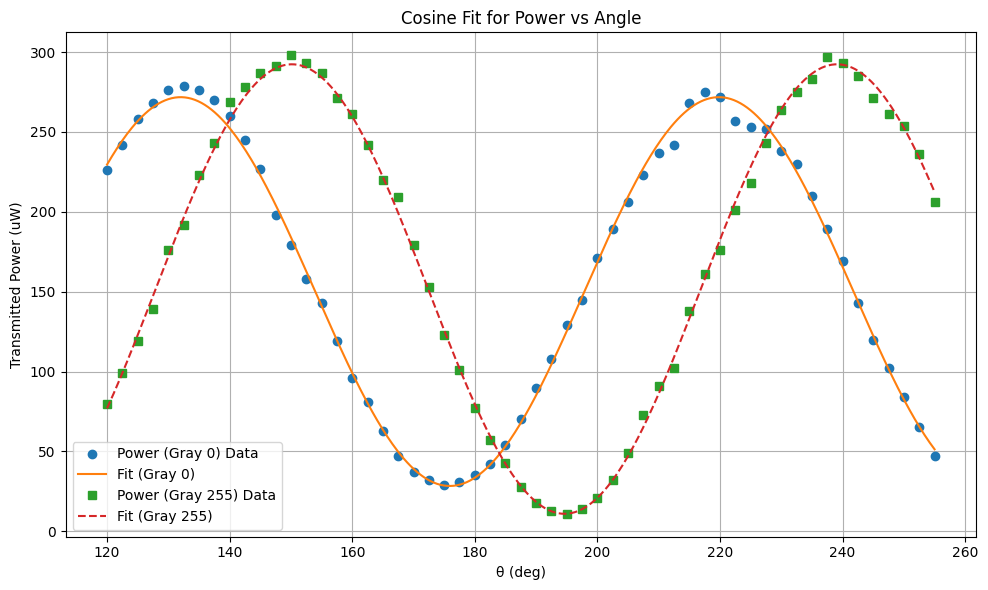
\includegraphics[width=0.4\textwidth]{半波片角度-功率图.png}
            \caption{不同灰度值下的角度-功率关系图}
            \label{fig:angle-power-relation}
            \end{figure}
图像如果用三角函数拟合,可以发现它们的相位大致相差66°。
对比度极大值位于为于170°,195°,对比度约为$P=|\frac{I_0-I_{255}}{I_0+I_{255}}|\approx 0.8$。


(2)测试 SLM 透过光功率随灰度变化曲线
将半波片角度固定于$\theta_m=170°$处,切换 SLM 输入图像的灰度值:
\begin{table}[H]
    \centering
\begin{tabular}{|c|c|c|c|}
\hline
灰度值 & $I_{out}$ & 灰度值 & $I_{out}$ \\
\hline
0 & 39.8 & 25 & 46.4 \\
\hline
50 & 54.6 & 75 & 64.2 \\
\hline
100 & 77.3 & 125 & 90.4 \\
\hline
150 & 105.5 & 175 & 122.1 \\
\hline
200 & 139.8 & 225 & 156.7 \\
\hline
250 & 172.5 &  &  \\
\hline
\end{tabular}

    \caption{灰度值与光功率关系表}
    \label{tab:gray-power-relation}
    \end{table}
画成图如下:
    \begin{figure}[H]
        \centering
        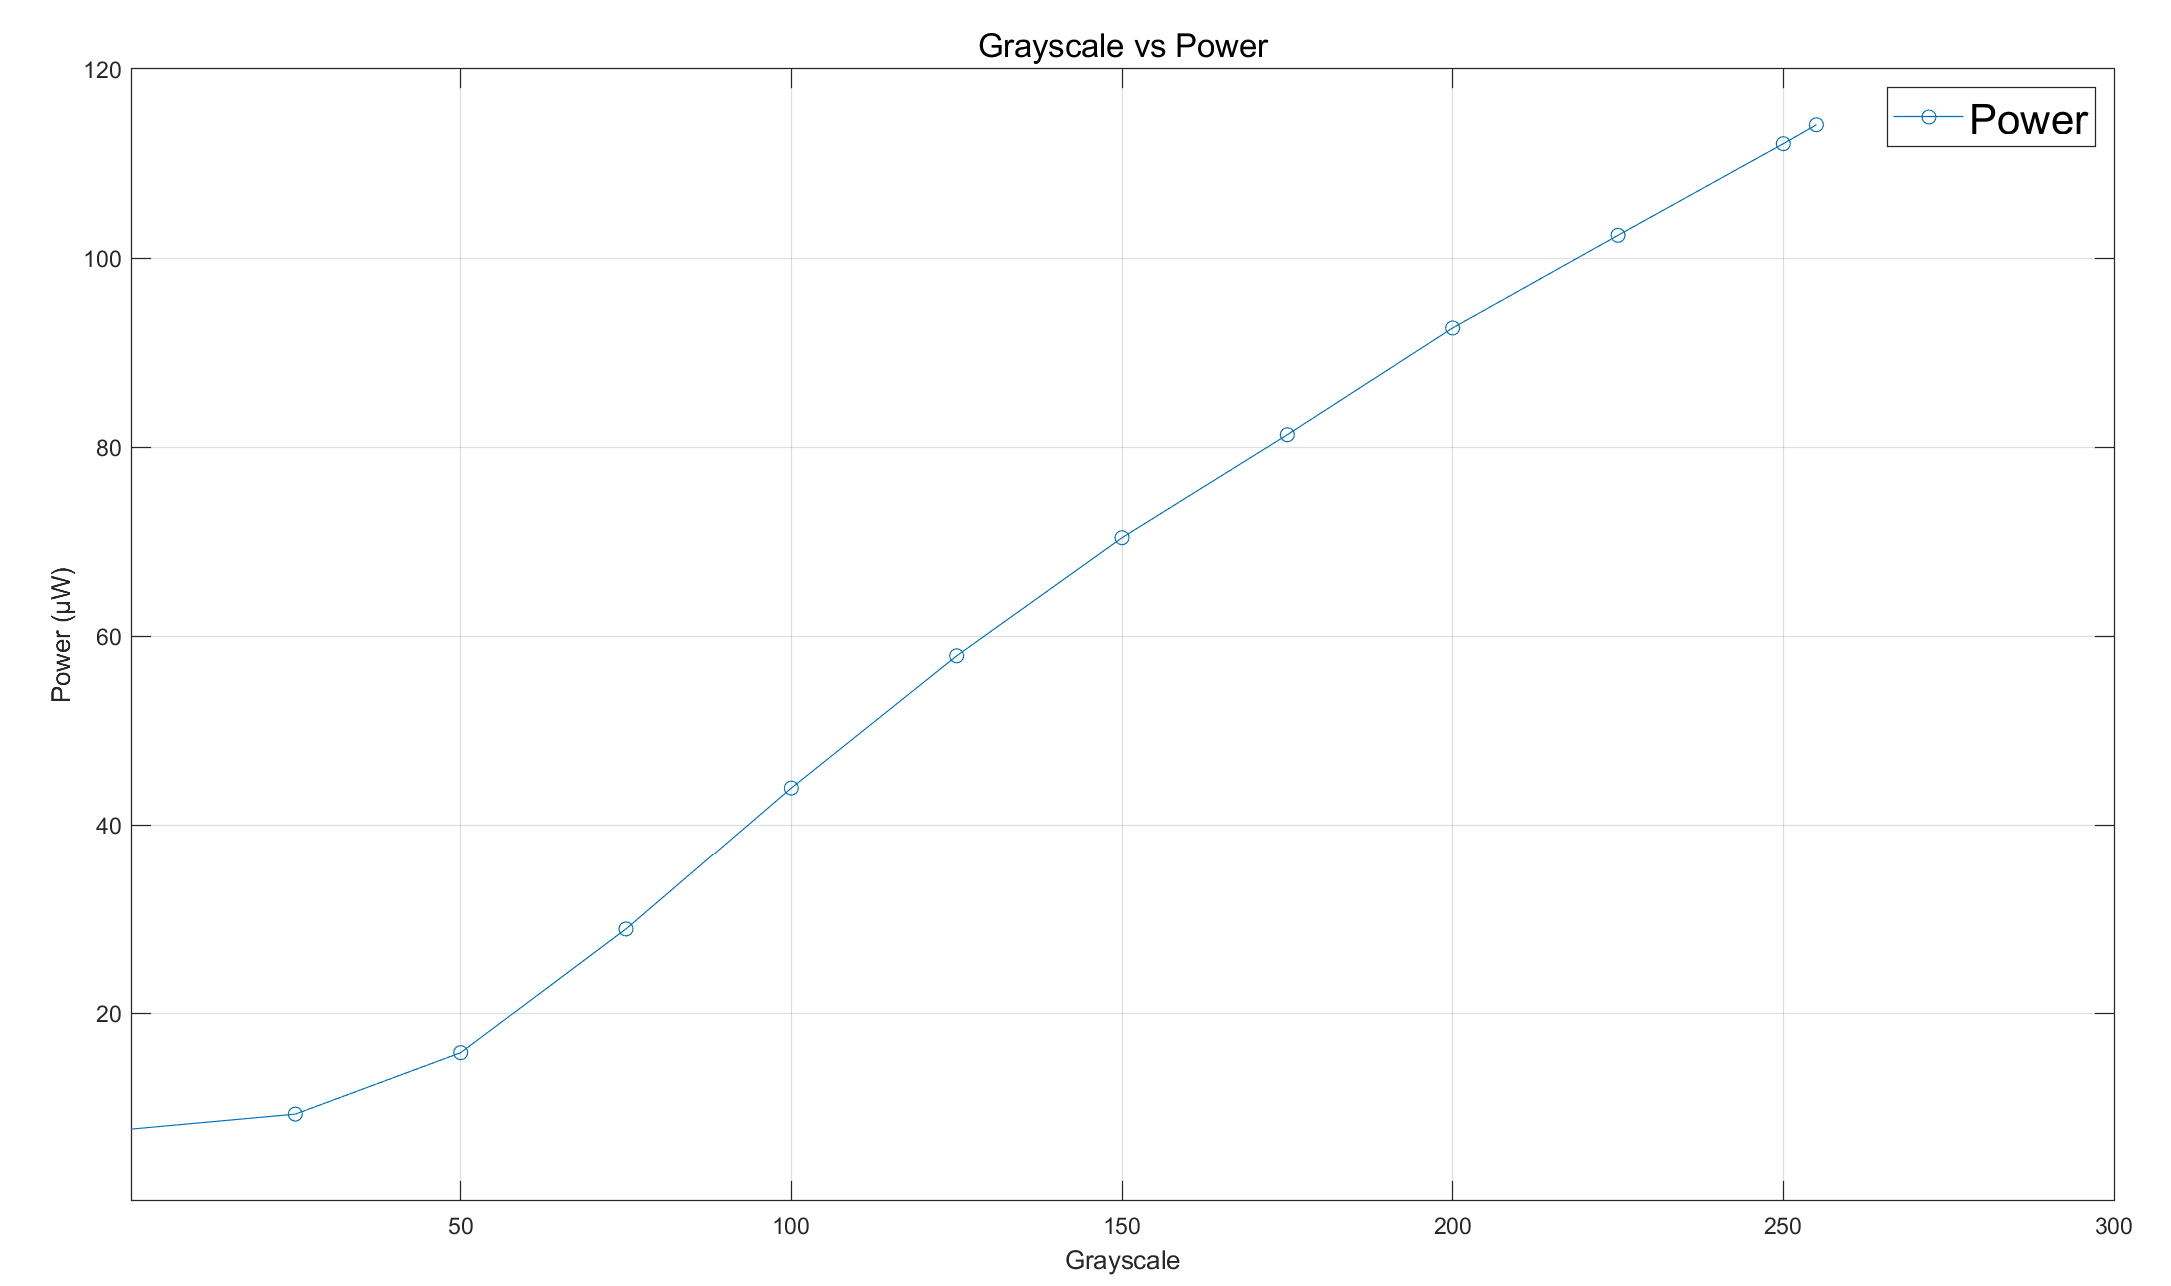
\includegraphics[width=0.4\textwidth]{灰度值-光功率图.png}
        \caption{灰度值与光功率关系图}
        \label{fig:gray-power-relation}
        \end{figure}
        可以发现光功率随灰度值的增加而增加;当灰度值在 0-50 区间时,光功率随灰度值的增
        加而增加的速度较慢,而在 50-250 区间,光功率随灰度值的增加而增加的速率稳定且较
        快。
\subsection{图像转换及黑栅效应的消除}
在实验 1 的基础上搭建光路,激光经扩束、准直后变为平行光,SLM、傅里叶透镜
1、光阑、傅里叶透镜 2 和 CMOS 按间隔为傅里叶透镜焦距 f=150mm 摆放。
实验过程中对照之前得到的角度-功率曲线,旋转半波片角度,观察不同角度的像(黑底白字的"H")的不同,用 CMOS 记录明显的正像(200°)、负像(170°),
以及边缘像(145°)如下图所示:
\begin{figure}[H]
    \centering
    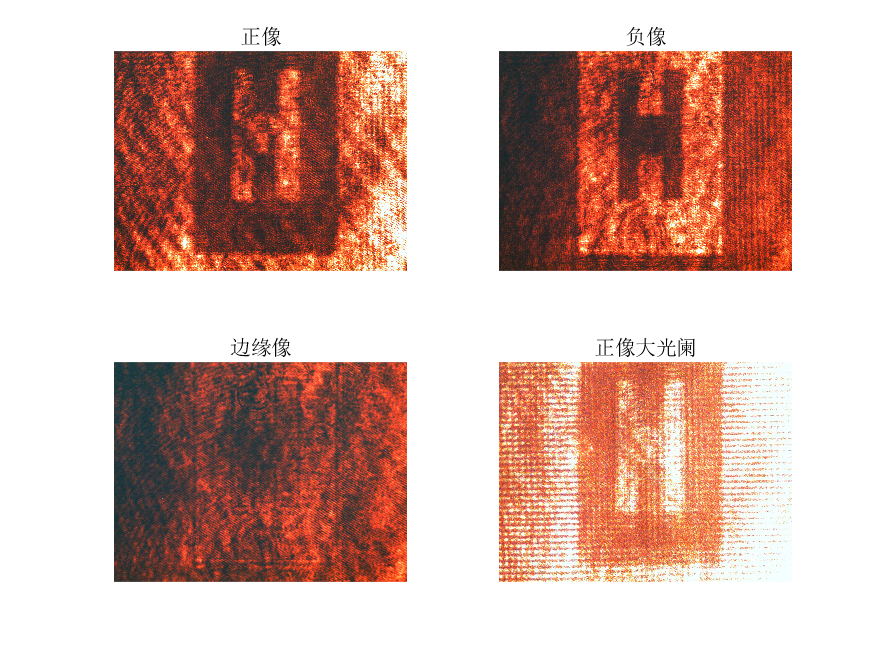
\includegraphics[width=0.4\textwidth]{图像排列.png}
    \caption{正像、负像、边缘像和正像大光阑}
    \label{fig:image-arrangement}
    \end{figure}
其中可见,光阑限制了图像的对比度。对于边缘像,由于灰度-强度映射不能够非常准确地定位出来,在合适的曝光时间下,图像灰度剧烈变化的地方仍然存在强度的差异,因此能观察到模糊的边缘。

\subsection{全息图的再现}
载入文件夹“SLM 图像”中的计算频谱图,处于汇聚透镜镜面的傅里叶全息图经过汇聚
透镜得到的衍射主极大,作傅里叶逆变换,再现的图像将出现在后焦面上,调整 CMOS 的位置,观察再现像:
\begin{figure}[H]
    \centering
    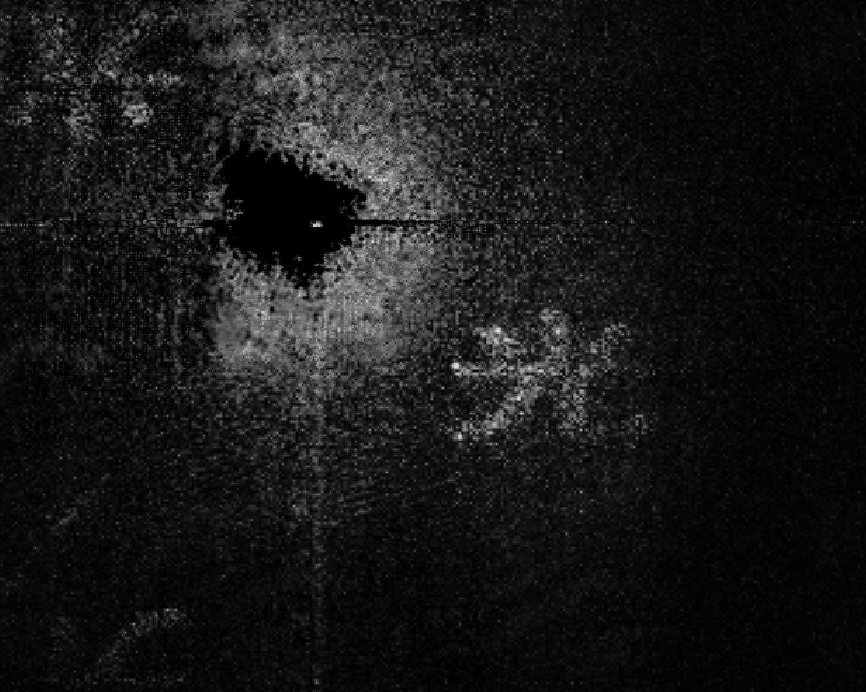
\includegraphics[width=0.4\textwidth]{reimage.png}
    \caption{再现像}
    \label{fig:reproduced-image}
    \end{figure}
在图中的四个象限中均可观察到“光”字,由于光路搭建不良,只有右下角的正再现像和右上角的倒再现像比较清晰。
\subsection{SLM 像素大小的测量}
把图中 CMOS 取下,换上白屏,即让白屏位于傅里叶透镜的焦平面上,根据透射光栅的
夫琅禾费衍射效应,测量 SLM 像素的尺寸。
根据夫琅禾费衍射公式
\begin{equation}
    a\sin{\theta}=n\lambda
\end{equation}
其中$\theta$可以用小角近似$\sin{\theta}=d/f$
测量焦平面的光斑的间距如下图

\begin{figure}[H]
    \centering
    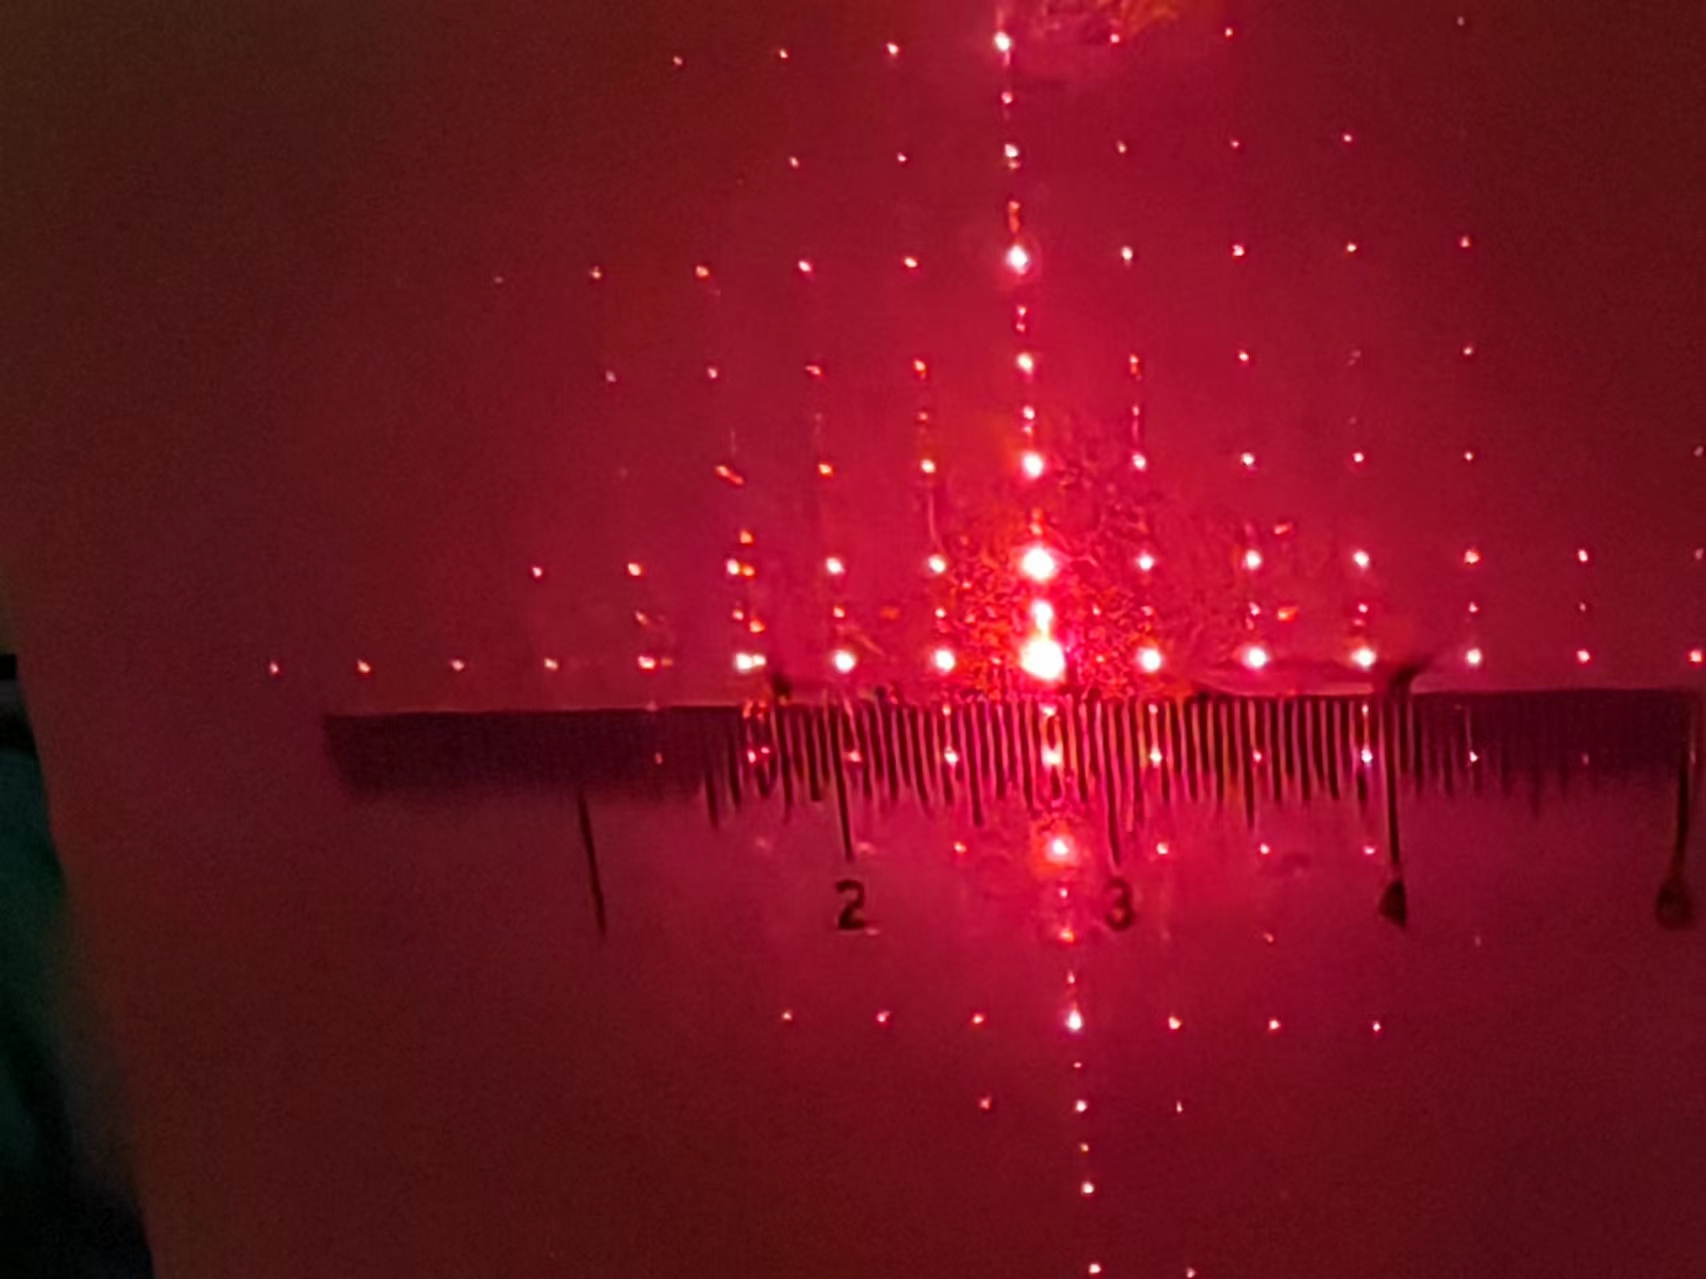
\includegraphics[width=0.4\textwidth]{衍射测量.jpg}
    \caption{衍射测量}
    \label{fig:diffraction-measurement}
    \end{figure}

有$d=3.6mm$。代入$f=15cm$和激光波长632.8nm,得
\begin{equation}
    a=2.72\times 10^4nm
\end{equation}

\section{总结和建议}
本实验实验使用由 He-Ne 激光器、起偏器、半波片、SLM、检偏器、探测器等元件组成
的光路及 CMOS 等来实现图像变换和全息图再现。实验测量得到的 SLM 像素的大小为
$2.72\times 10^4nm$。
实验过程需要注意组成光路的各个元件必须满足等高共轴,部分元件之间的距离要满足
所给的焦距要求。
\end{multicols}
\section{附录}
\subsection{实验数据}
\begin{figure}[H]
	\centering
	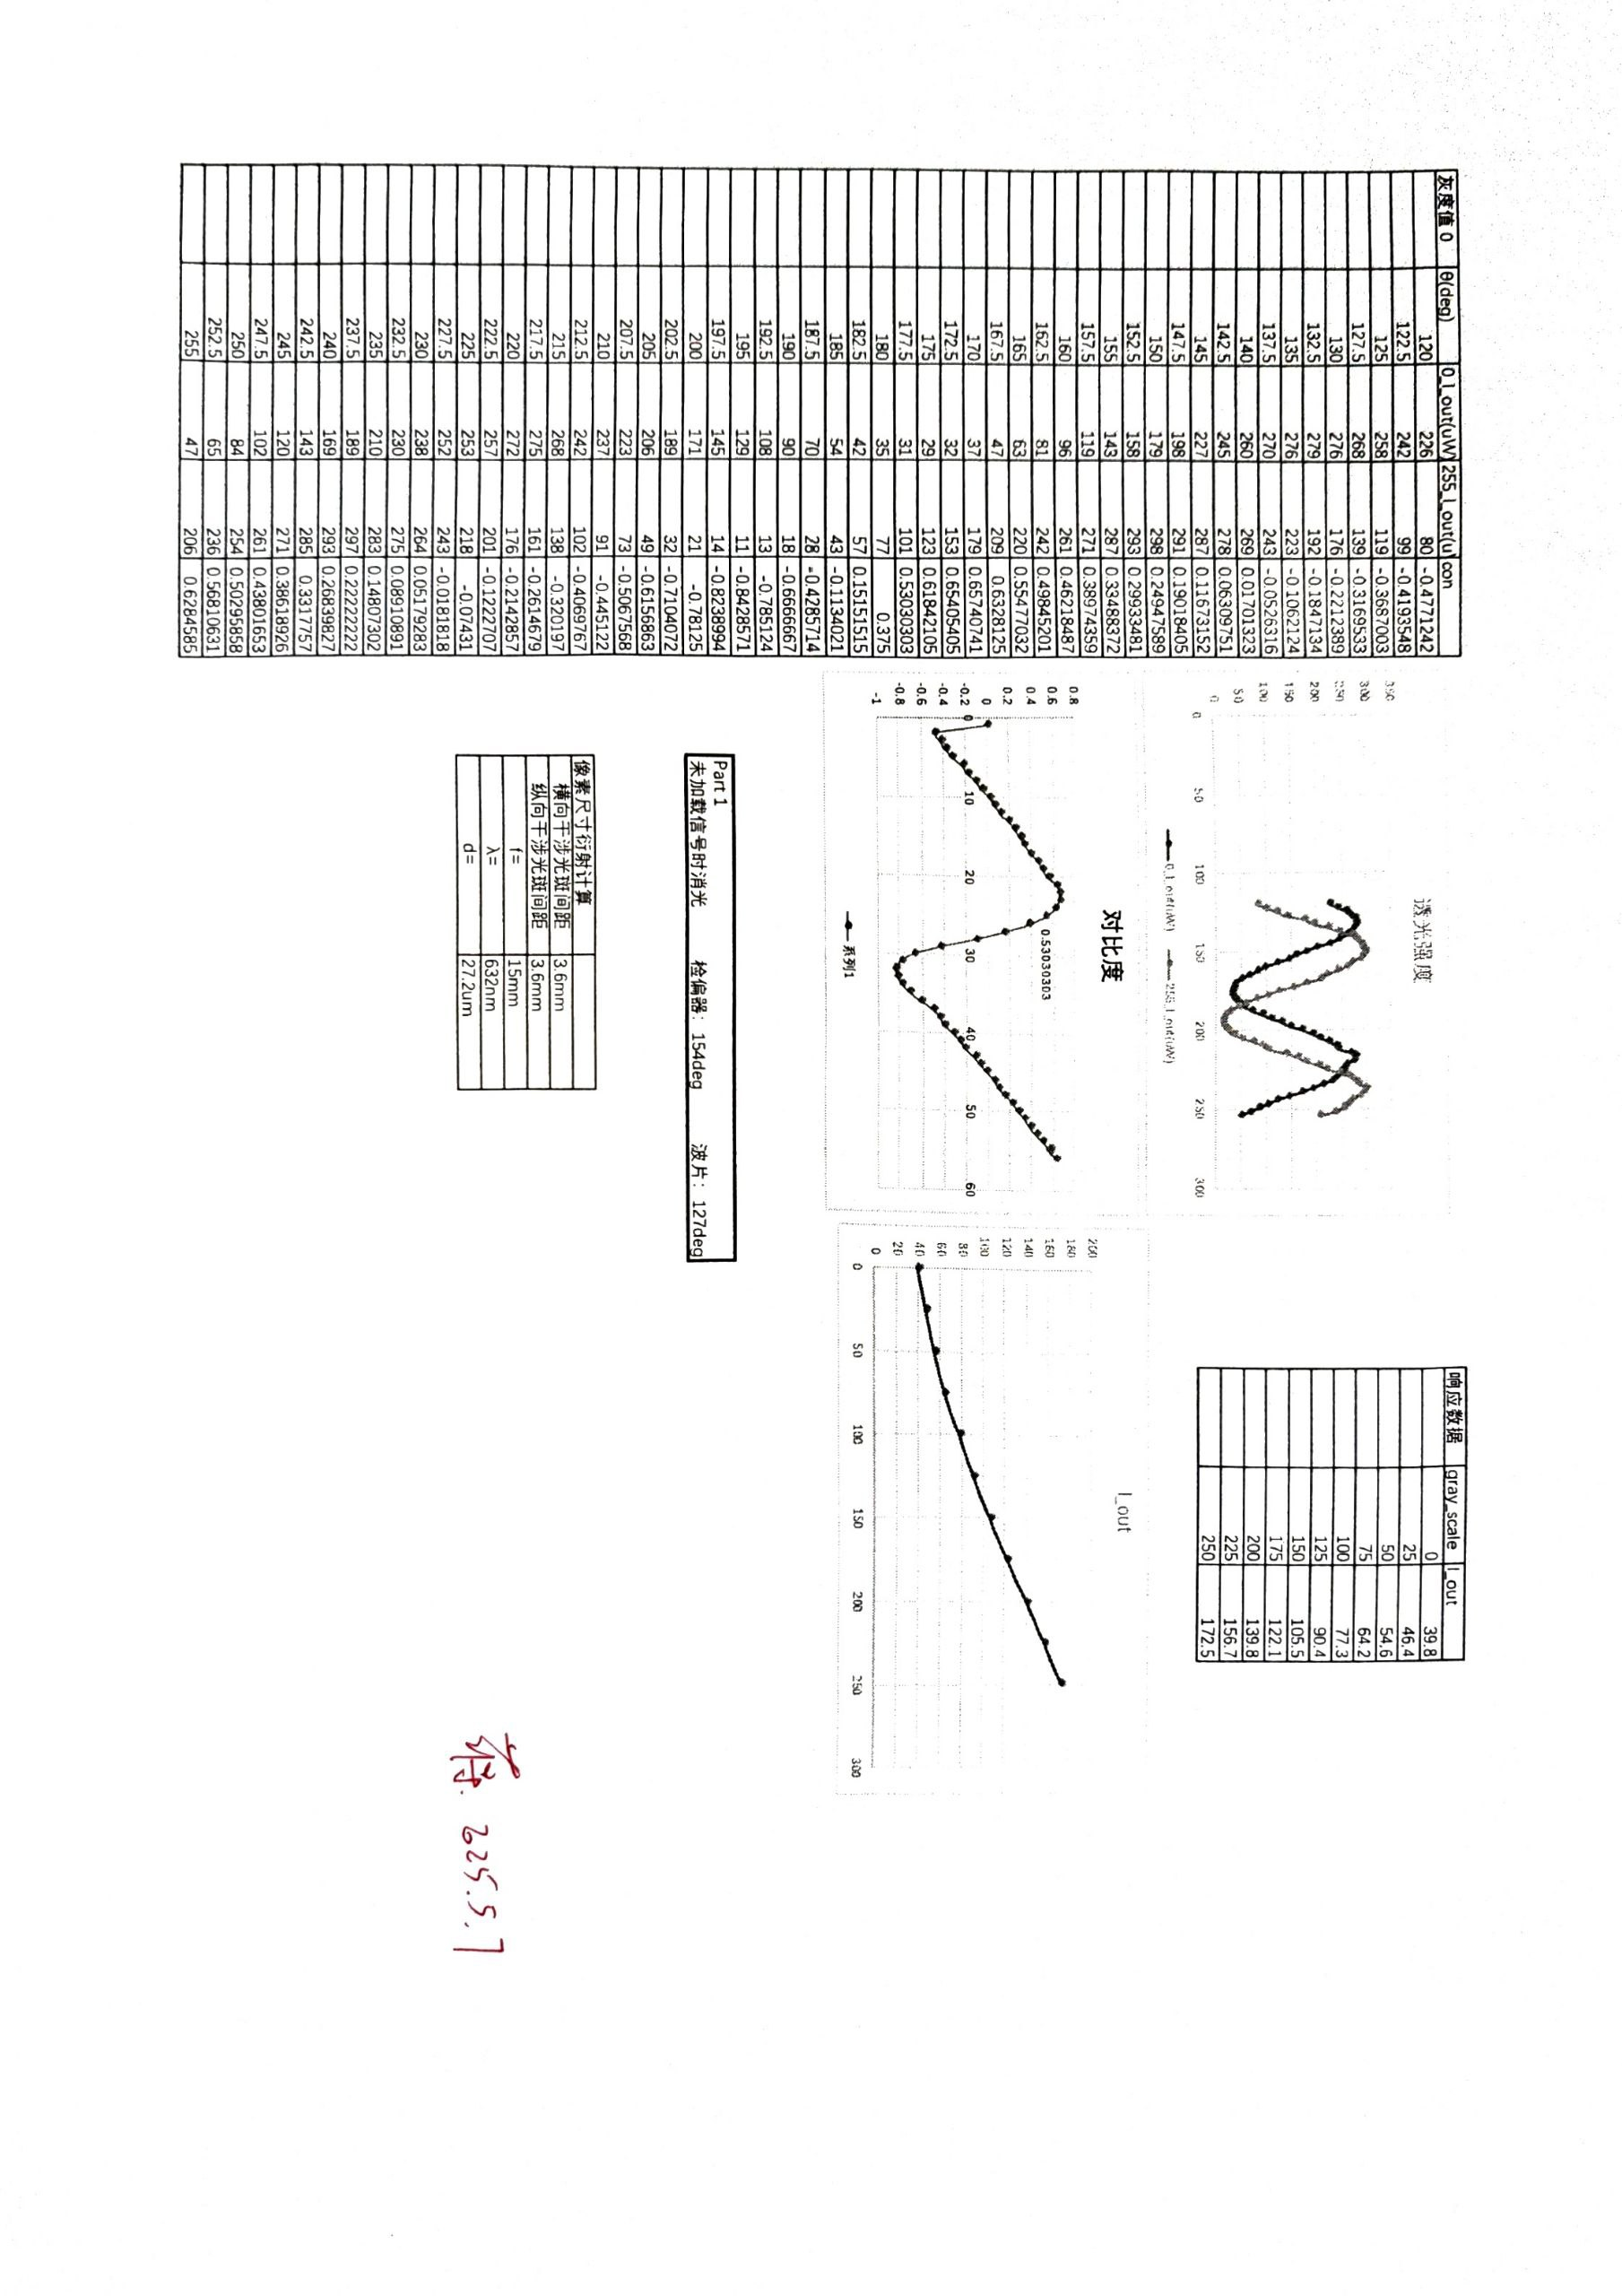
\includegraphics[width=\textwidth]{data.jpg}
	\caption{实验数据}
	\label{fig:experiment-data}
\end{figure}



\end{document}
